\chapter{Conclusion}

\paragraph*{}
In summary, the project is making steady progress with many core modules demon-
strated in simulation. While some completed components may need further refinement
to accommodate dependencies from other subsystems, the current state is aligned with
our objectives. As we proceed, our efforts will follow two main paths in parallel.

On one track, we will test and enhance the Graph SLAM algorithm within the We-
bots simulation environment. This testing phase will help evaluate the algorithm’s
performance under conditions closely resembling real-world scenarios and guide any
necessary improvements.

Concurrently, another part of the team will shift focus towards hardware develop-
ment. This involves finalising 3D designs for the robot’s physical components, ensur-
ing they meet the required specifications. Once the designs are ready, the team will
move on to integrating various elements like sensors, actuators, and computational
units. See Figure \ref{fig:future-plans} for a the visualisation of the additional step to our flow

\begin{figure} [H]
    \centering
    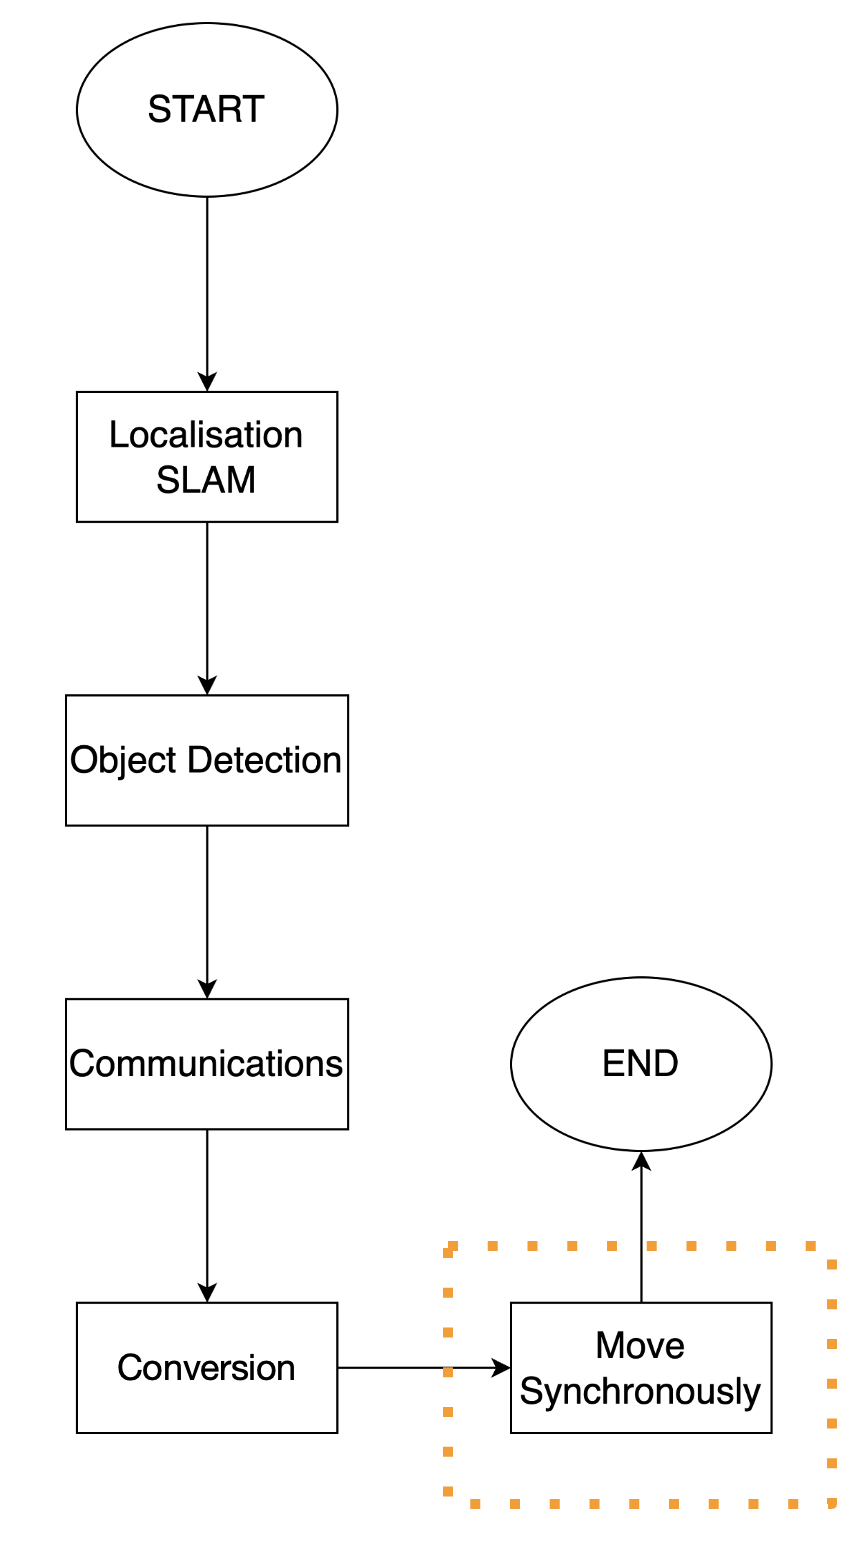
\includegraphics[width=0.5\linewidth]{assets/images/conclusion/future-plans.png}
    \caption{Future plans for the project}
    \label{fig:future-plans}
\end{figure}

By advancing both software and hardware components simultaneously, we aim to
achieve a fully integrated and functioning platform. This dual approach will ensure
that our final system is both robust and reliable, setting the foundation for seamless
transition from simulation to real-world implementation.